\PassOptionsToPackage{table}{xcolor}
%\documentclass{beamer}
\documentclass[compress]{beamer}
%\usetheme{Epam}
\usetheme{Copenhagen}
\usepackage{xcolor}
\usepackage{listings}
\usepackage{graphicx}
\usepackage[utf8]{inputenc}
\usepackage{datetime}
\usepackage{beamerthemesplit}
%\beamertemplatenavigationsymbolsempty
\usepackage{listingsutf8}
\usepackage{ragged2e}
\usepackage{hyperref}
\lstset{ %
  language=C,                      % the language of the code
%  basicstyle=\ttfamily,           % the size of the fonts that are used for the code
%  basicstyle=\ttfamily\tiny,      % the size of the fonts that are used for the code
  basicstyle=\ttfamily\scriptsize, % the size of the fonts that are used for the code
  numbers=left,                    % where to put the line-numbers
  numberstyle=\tiny\color{gray},   % the style that is used for the line-numbers
  stepnumber=1,                    % the step between two line-numbers. If it's 1, each line 
                                   % will be numbered
  numbersep=5pt,                   % how far the line-numbers are from the code
  %backgroundcolor=\color{gray},   % choose the background color. You must add \usepackage{color}
  showspaces=false,               % show spaces adding particular underscores
  showstringspaces=false,         % underline spaces within strings
  showtabs=false,                 % show tabs within strings adding particular underscores
%  frame=shadowbox,                   % adds a frame around the code
  rulecolor=\color{black},        % if not set, the frame-color may be changed on line-breaks within not-black text (e.g. commens (green here))
  tabsize=4,                      % sets default tabsize to 4 spaces
  captionpos=,                   % sets the caption-position to bottom
  breaklines=false,                % sets automatic line breaking
  breakatwhitespace=false,        % sets if automatic breaks should only happen at whitespace
  title=\lstname,                 % show the filename of files included with \lstinputlisting;
                                  % also try caption instead of title
  keywordstyle=\color{blue},      % keyword style
  commentstyle=\color{mygreen},   % comment style
  stringstyle=\color{magenta},    % string literal style
%  escapeinside={\%*}{*)},        % if you want to add a comment within your code
  inputencoding=utf8,
  extendedchars=\true,
  morekeywords={*,..., restrict, alignof, alignas, bool, true, false, size_t, ssize_t, inline, \_Noreturn, noreturn},
  breakautoindent=false,
  breakindent=1pt,
}

%\setbeameroption{show only notes}
%\usepackage{pgfpages}
%\setbeameroption{show notes}
%\setbeameroption{show notes on second screen=right}

\setbeamertemplate{navigation symbols}{}

\definecolor{oddrow}{RGB}{100,149,237}
\definecolor{evenrow}{RGB}{135,206,250}
\def\mybs{\textbackslash}
\newcommand{\qq}{\symbol{34}} % the decimal ascii code for "
\newcommand{\sq}{\symbol{39}} % the decimal ascii code for '

\makeatletter
\newcommand{\rmnum}[1]{\romannumeral #1}
\newcommand{\Rmnum}[1]{\expandafter\@slowromancap\romannumeral #1@}
\newcommand{\inc}{\symbol{45}\symbol{45}}
\newcommand{\dec}{\symbol{43}\symbol{43}}
\newcommand{\lsh}{\symbol{60}\symbol{60}}
\newcommand{\rsh}{\symbol{62}\symbol{62}}
\makeatother

\newcommand{\specialcell}[2][c]{%
  \begin{tabular}[#1]{@{}c@{}}#2\end{tabular}}
\newcommand{\specialcellhl}[2][l]{%
  \begin{tabular}[#1]{@{}l@{}}#2\end{tabular}}
\newcommand{\specialcellhc}[2][c]{%
  \begin{tabular}[#1]{@{}c@{}}#2\end{tabular}}

\definecolor{mygreen}{rgb}{0,0.6,0}
\definecolor{olive}{rgb}{0.3, 0.4, .1}
\definecolor{fore}{RGB}{249,242,215}
\definecolor{back}{RGB}{51,51,51}
\definecolor{title}{RGB}{255,0,90}
\definecolor{dgreen}{rgb}{0.,0.6,0.}
\definecolor{gold}{rgb}{1.,0.84,0.}
\definecolor{JungleGreen}{cmyk}{0.99,0,0.52,0}
\definecolor{BlueGreen}{cmyk}{0.85,0,0.33,0}
\definecolor{RawSienna}{cmyk}{0,0.72,1,0.45}
\definecolor{Magenta}{cmyk}{0,1,0,0}

\newcommand{\kwblue}[1]{\texttt{\textcolor{blue}{#1}}}
\newcommand{\kwblack}[1]{\texttt{\textcolor{black}{#1}}}
\newcommand{\kwred}[1]{\texttt{\textcolor{red}{#1}}}
\newcommand{\kwmagenta}[1]{\texttt{\textcolor{Magenta}{#1}}}

%\newcommand{\hdr}[1]{\textless{#1}\textgreater{}}
\newcommand{\hdr}[1]{\textless{\kwmagenta{#1}}\textgreater{}}

\author[\href{mailto:vasili_slapik@epam.com}{Vasili Slapik}]{\texorpdfstring{Vasili Slapik\newline\href{mailto:vasili_slapik@epam.com}{vasili\_slapik@epam.com}}{Vasili Slapik}}


\title{\Rmnum{1}. Introduction}

\begin{document}

%%%%%%%%%%%%%%%%%%%%%%%%%%%%%%%%%%%%%%%%%%%%%%%%%%%%%%%%%%%%%%%%%%%%%%%%%%%%%%%%%
% 0. Intro
% 1. What the course is about
%    - new features (c89,c99,c11)
%    - the course is rather about how not to write instead of how to write
%    - traps/common mistakes, etc.
% 2. Why English
% 3. Linux, only Linux
% 4. Audience: refresh/deepen knowledge, a bit challanging for newcomers
% 5. Strongly suggest implementing practical task
% 6. Timetable (10 lectures + 1 lecture for practice analyze) around 1:40 each

%%%%%%%%%%%%%%%%%%%%%%%%%%%%%%%%%%%%%%%%%%%%%%%%%%%%%%%%%%%%%%%%%%%%%%%%%%%%%%%%%
\frame{\titlepage}
%%%%%%%%%%%%%%%%%%%%%%%%%%%%%%%%%%%%%%%%%%%%%%%%%%%%%%%%%%%%%%%%%%%%%%%%%%%%%%%%%
\begin{frame}{C main steps}
    \begin{itemize}
        \note{Miltics 1964; MIT, GE, Bell Labs; concept of file, virtual memory, dynamic linking; PL/1}
        \note{Unix end of 196x; Bell Labs; concept of file, virtual memory, dynamic linking; PL/1}
        \item 1969 - 1973: developed by Dennis Ritchie at AT\&T Bell Labs.
        \pause\item 1978: Brian Kernighan and Dennis Ritchie published the first edition of The C Programming Language (K\&R).
        \pause\item 1989: the C standard ratified as ANSI X3.159-1989 "Programming Language C" (ANSI C or C89).
        \pause\item 1990: approved by the ISO as an international standard (C90).
        \pause\item 1999: revised standart by ISO (C99).
        \pause\item 2011: the current version approved by ISO (C11).
    \end{itemize}
\end{frame}
%%%%%%%%%%%%%%%%%%%%%%%%%%%%%%%%%%%%%%%%%%%%%%%%%%%%%%%%%%%%%%%%%%%%%%%%%%%%%%%%%
\begin{frame}{Dennis Ritchie, 1941 - 2011}
    \begin{center}
        \only<1>{
            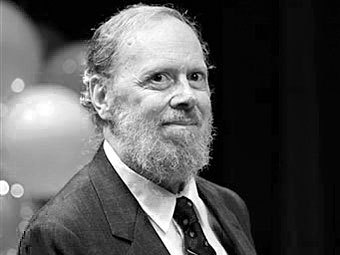
\includegraphics[height=7cm]{richie.png}
        }
        \only<2>{
            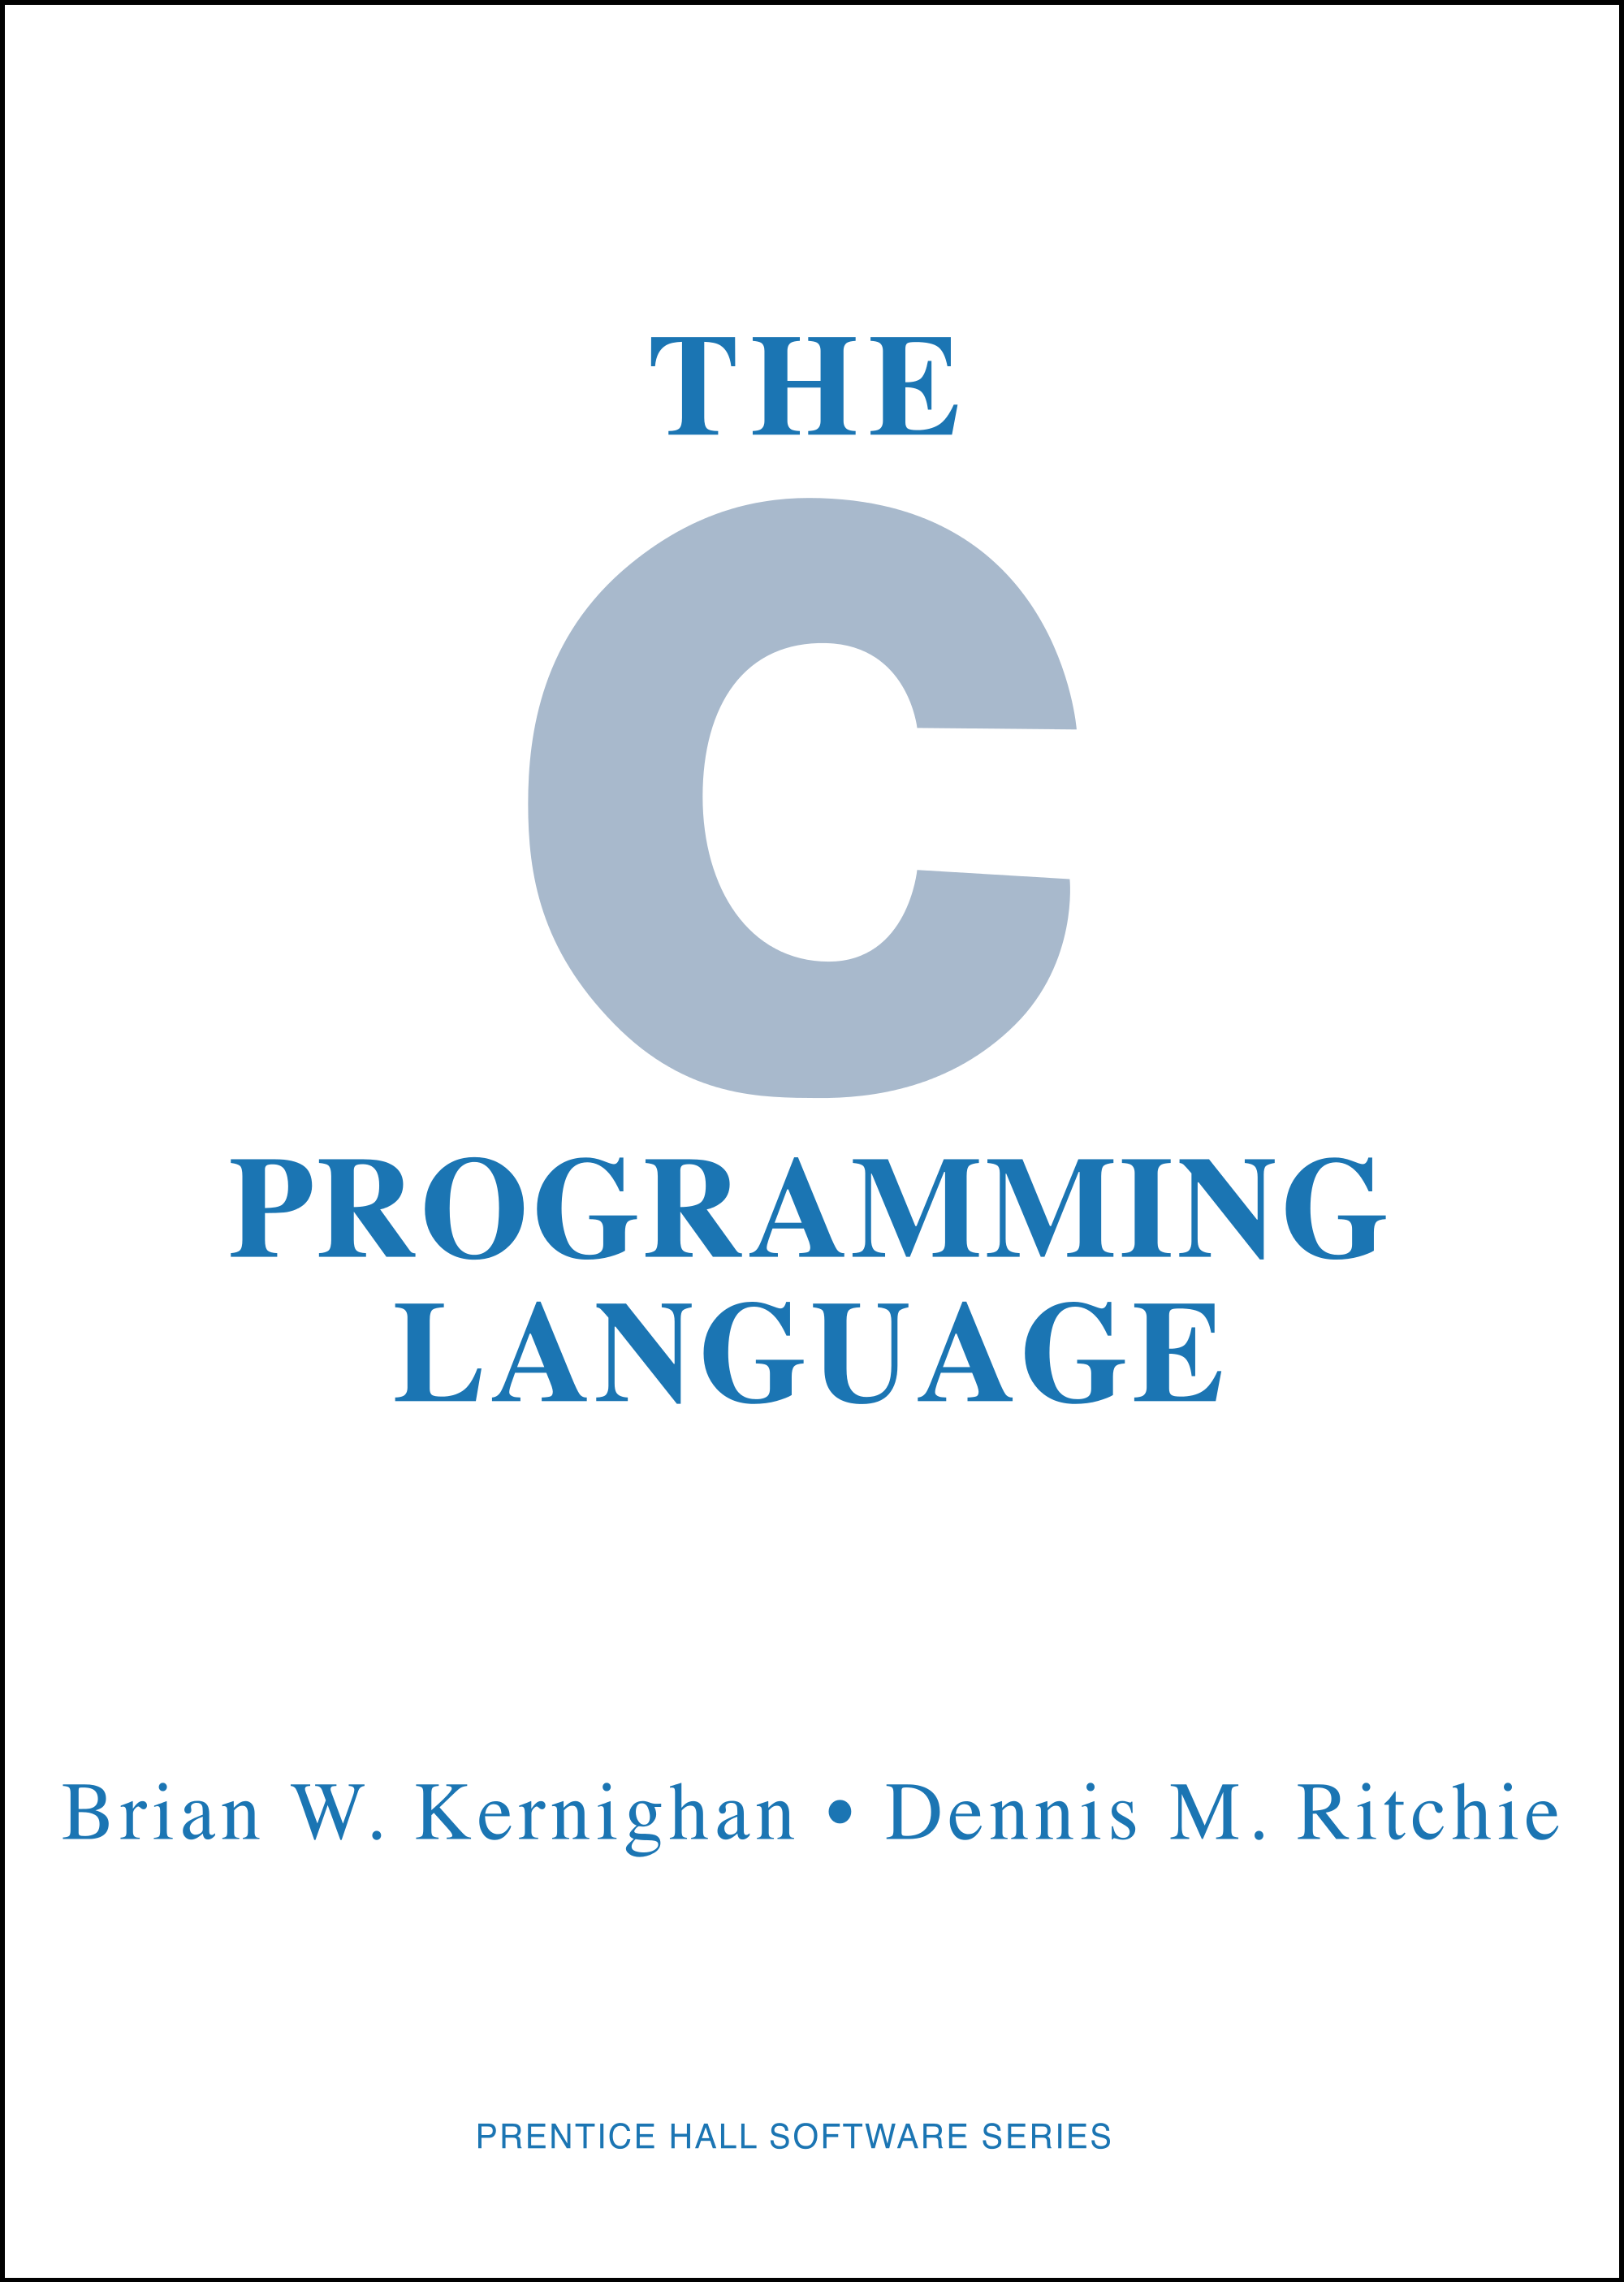
\includegraphics[height=7cm]{KandR_book.png}
        }
        \only<3>{
            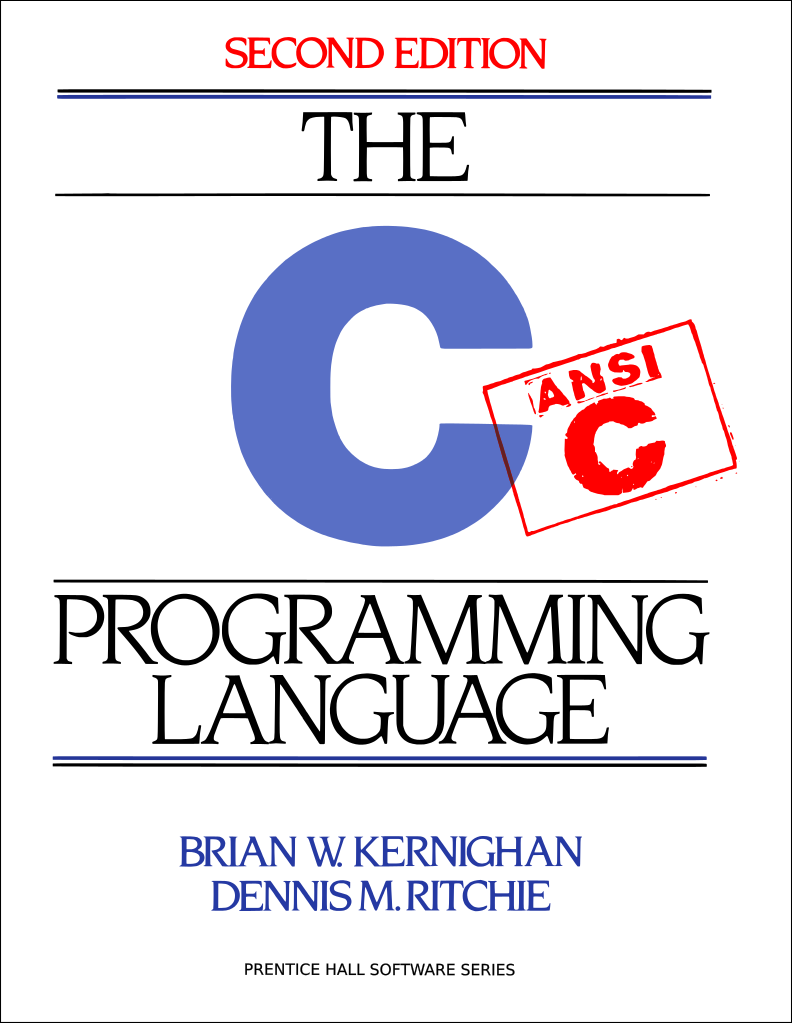
\includegraphics[height=7cm]{KandR_book2.png}
        }
    \end{center}
\end{frame}
%%%%%%%%%%%%%%%%%%%%%%%%%%%%%%%%%%%%%%%%%%%%%%%%%%%%%%%%%%%%%%%%%%%%%%%%%%%%%%%%%
\begin{frame}{Position in TIOBE index}
    \begin{center}
%        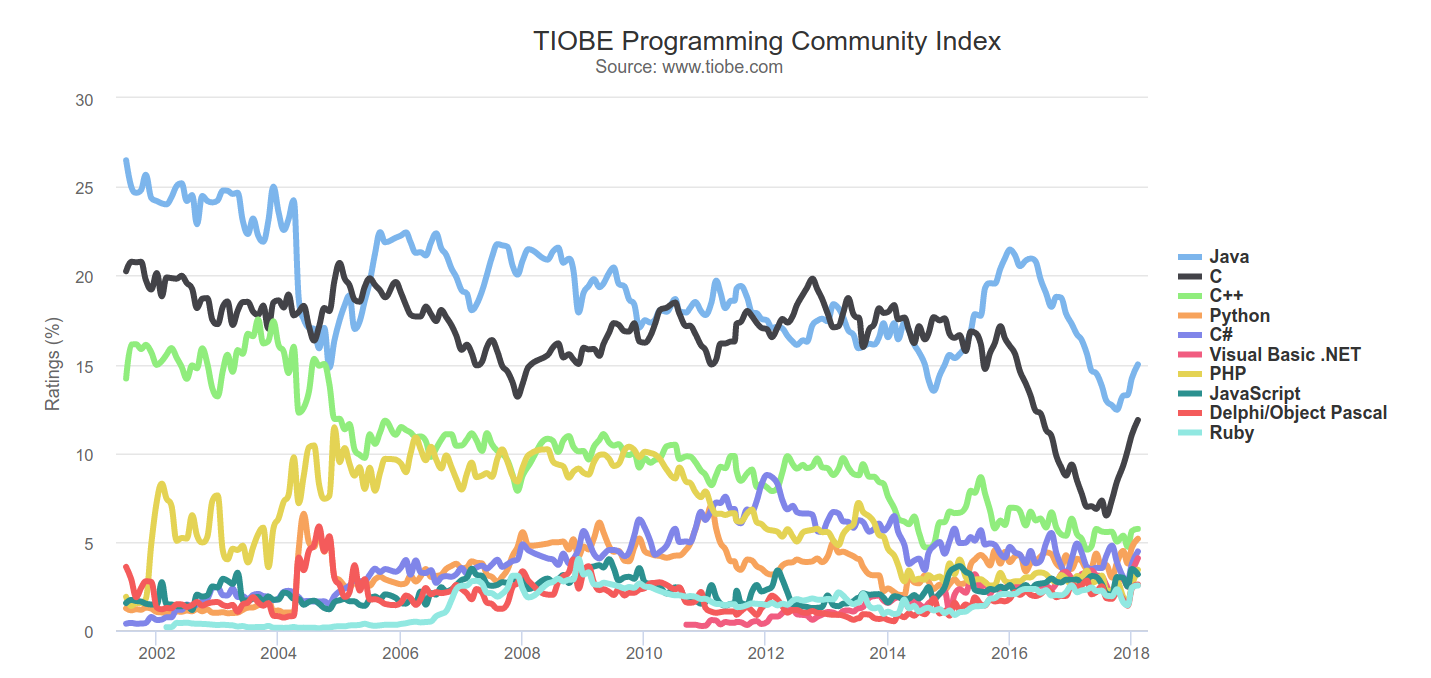
\includegraphics[height=7cm]{tiobe_4.png}
        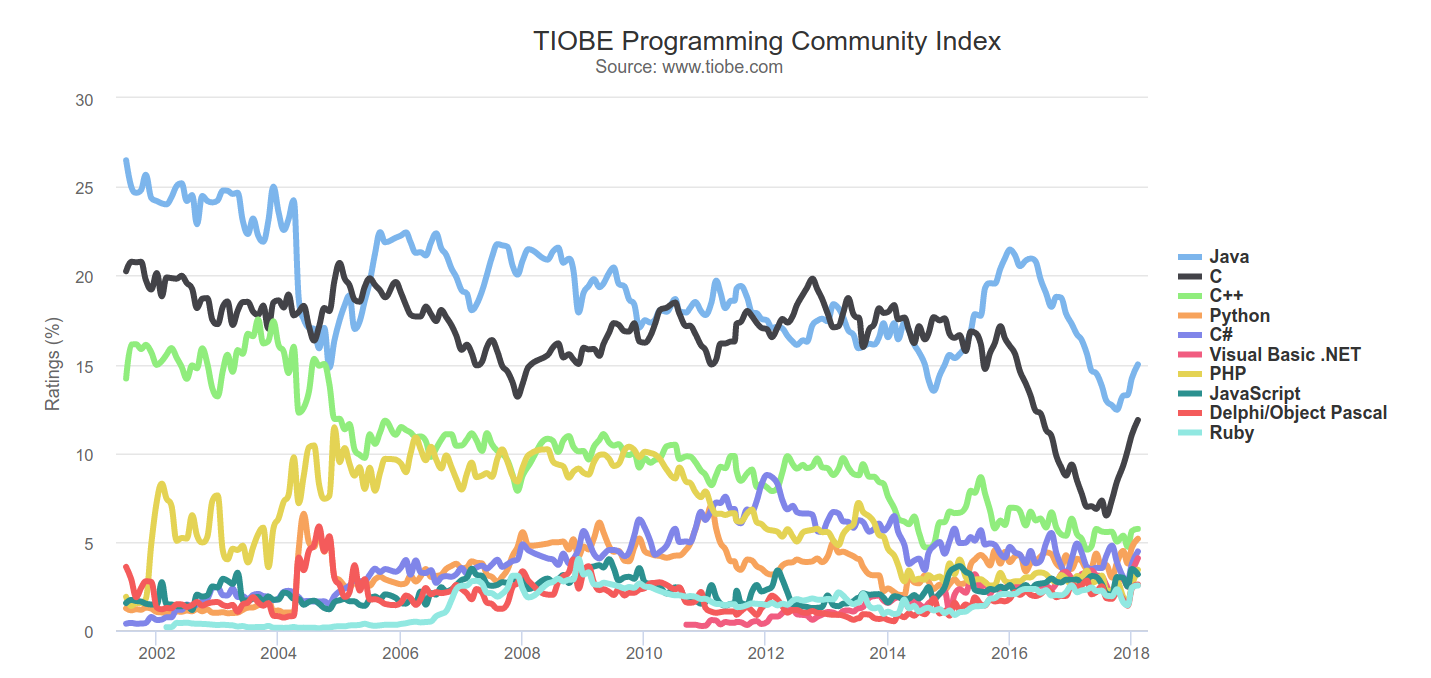
\includegraphics[width=11cm]{tiobe_4.png}
    \end{center}
\end{frame}
%%%%%%%%%%%%%%%%%%%%%%%%%%%%%%%%%%%%%%%%%%%%%%%%%%%%%%%%%%%%%%%%%%%%%%%%%%%%%%%%%
\begin{frame}{Spirit of C}
    \begin{itemize}
        \item Trust the programmer.
        \pause \item Don’t prevent the programmer from doing what needs to be done.
        \pause \item Keep the language small and simple.
        \pause \item Provide only one way to do an operation.
        \pause \item Make it fast, even if it is not guaranteed to be portable.
    \end{itemize}
\end{frame}
%%%%%%%%%%%%%%%%%%%%%%%%%%%%%%%%%%%%%%%%%%%%%%%%%%%%%%%%%%%%%%%%%%%%%%%%%%%%%%%%%
\begin{frame}{Languages based on C}
    \begin{center}
        \includegraphics[height=7cm]{tree.png}
    \end{center}
\end{frame}
%%%%%%%%%%%%%%%%%%%%%%%%%%%%%%%%%%%%%%%%%%%%%%%%%%%%%%%%%%%%%%%%%%%%%%%%%%%%%%%%%
\begin{frame}{Creation of executable module}
    \begin{center}
        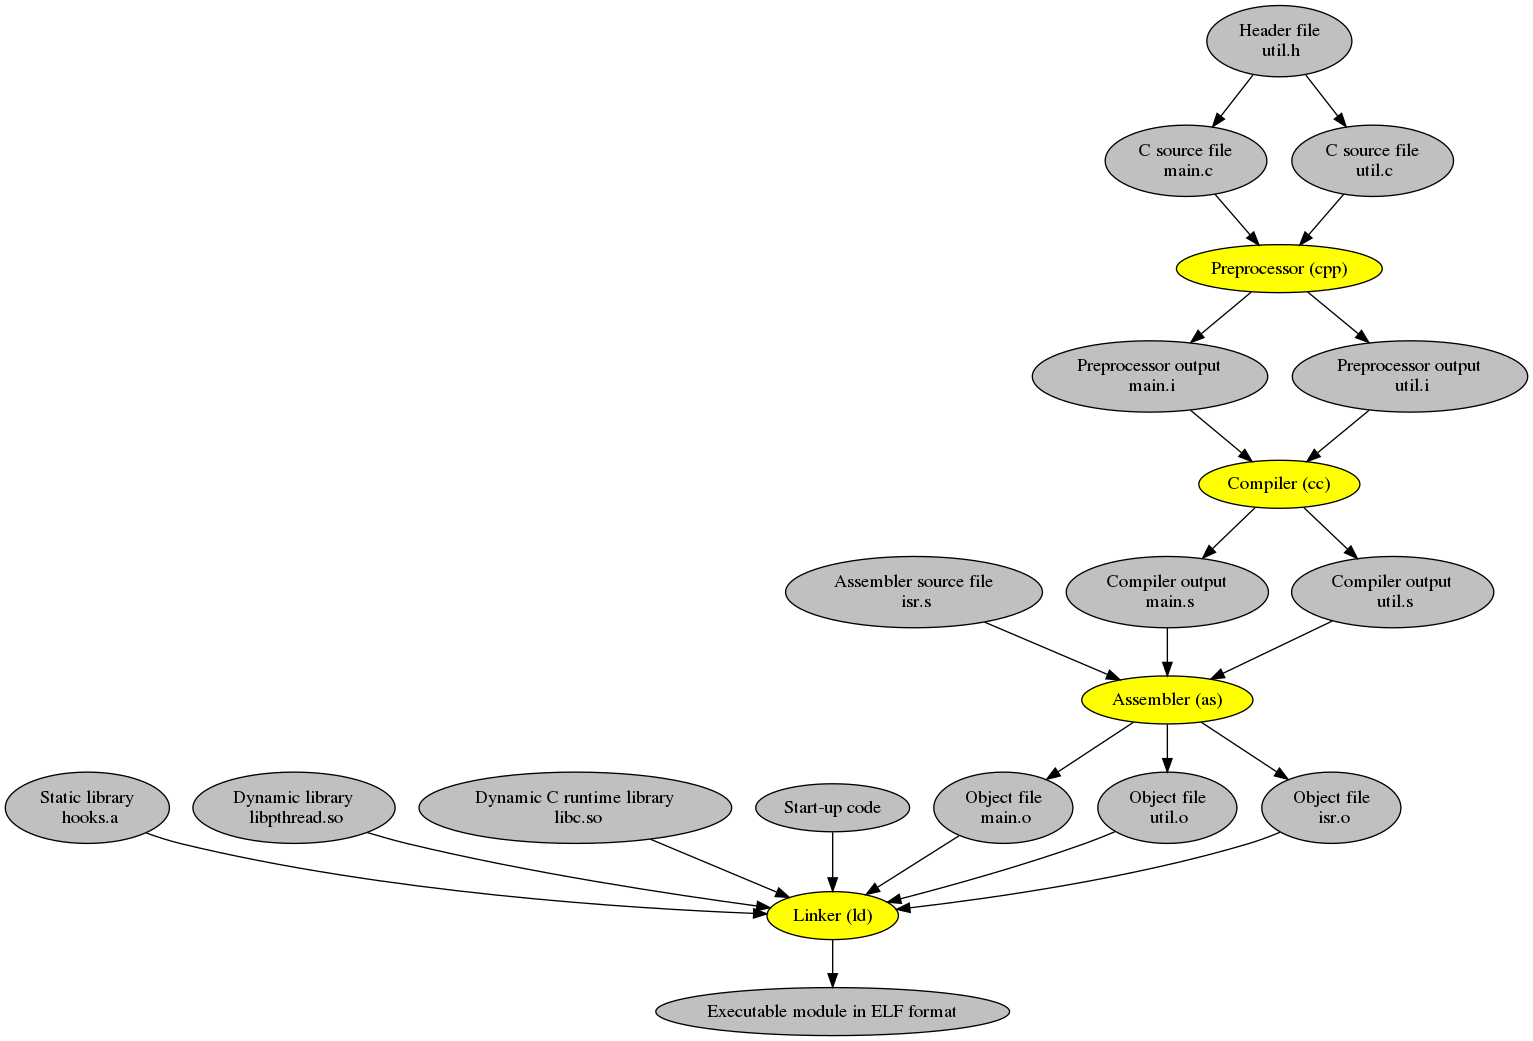
\includegraphics[height=7cm]{01_flow.png}
    \end{center}
\end{frame}
%%%%%%%%%%%%%%%%%%%%%%%%%%%%%%%%%%%%%%%%%%%%%%%%%%%%%%%%%%%%%%%%%%%%%%%%%%%%%%%%%
\begin{frame}[fragile]{GCC most frequent options}
    \only<1>{
        \lstinputlisting[breaklines,numbers=none,language=]{01_gcc_options.txt}
    }
    \only<2>{
        \begin{center}
        \scriptsize{
        \rowcolors{1}{oddrow}{evenrow}
        \begin{tabular}{ll}
            \texttt{-c}            & \specialcellhl{Compile or assemble the source files, but do not link; \\
                                        the output is object files.} \\
            \texttt{-S}            & Compile only; output assembly code. \\
            \texttt{-E}            & Pre-process only; output pre-processed code. \\
            \texttt{-std=standart} & \specialcellhl{Determine the language standard; could be but not limited to\\
                                        \texttt{c89}, \texttt{c99}, \texttt{c11}, \texttt{gnu11} (default).} \\
            \texttt{-g}            & Produce debug information. \\
            \texttt{-pg}           & \specialcellhl{Generate extra code to write profile information \\
                                        suitable for the analysis program gprof.} \\
            \texttt{-Olevel}       & Optimization level from \texttt{0} (default) to \texttt{3}; also can be \texttt{-Ofast}, \texttt{-Os}.\\
            \texttt{-Wwarn}        & \specialcellhl{Enable \texttt{warn} warning; frequently used are: \\
                                        \texttt{all}, \texttt{pedantic}, \texttt{error}, \texttt{format}.} \\
            \texttt{-llibrary}     & \specialcellhl{Links to a standard library; use -lm for maths library (libm.so).} \\
            \texttt{-Dmacro}       & Define a macro, one can also use \texttt{-Dmacro=val}. \\
            \texttt{-Umacro}       & \specialcellhl{Undefine any previous definition of name, either built-in \\
                                        or provided with a \texttt{-D} option.} \\
            \texttt{-Idir}         & \specialcellhl{Add the directory dir to the head of the list of directories \\
                                        to be searched for header files.} \\
            \texttt{-Ldir}         & \specialcellhl{Add directory \texttt{dir} to the list of directories to be searched for \texttt{-l}.} \\
            \texttt{@file}         & Read command-line options from file. \\
            \texttt{-save-temps}   & Save intermediate files in the current directory. \\

        \end{tabular}
        }
        \end{center}
    }

\end{frame}
%%%%%%%%%%%%%%%%%%%%%%%%%%%%%%%%%%%%%%%%%%%%%%%%%%%%%%%%%%%%%%%%%%%%%%%%%%%%%%%%%
\begin{frame}{Hello world!}
    \lstinputlisting{01_hello_world.c}
\end{frame}
%%%%%%%%%%%%%%%%%%%%%%%%%%%%%%%%%%%%%%%%%%%%%%%%%%%%%%%%%%%%%%%%%%%%%%%%%%%%%%%%%
% It is very common for people to say — or at least think — something like this:
%
% The x86 ADD instruction is used to implement C’s signed add operation, and it
% has two’s complement behavior when the result overflows. I’m developing for
% an x86 platform, so I should be able to expect two’s complement semantics when
% 32-bit signed integers overflow.
%
% THIS IS WRONG. You are saying something like this:
%
% Somebody once told me that in basketball you can’t hold the ball and run.
% I got a basketball and tried it and it worked just fine. He obviously ddn’t
% understand basketball.
\begin{frame}{Undefined, unspecified, implementation-defined behaviour}
    \only<1>{
        \justifying
            The terms unspecified behavior, undefined behavior, and implementation-defined behavior are
        used to categorize the result of writing programs whose properties the Standard does not, or
        cannot, completely describe.

    }
    \only<2>{
        \begin{block}{Unspecified behaviour:}
            \justifying
            behavior where the standard provides two or more possibilities and imposes no further
            requirements on which is chosen in any instance.

        \end{block}
        \lstinputlisting{01_unspec_b.c}
    }
    \only<3>{
        \begin{block}{Implementation defined behavour:}
            \justifying
            unspecified behavior where each implementation documents how the choice is made.

        \end{block}
        \lstinputlisting{01_implem_def_b.c}
    }
    \only<4>{
        \note{Abstract C machine: each operation performed by the program is either defined or undefined}
        \begin{block}{Undefined behaviour:}
            \justifying
            behavior, upon use of a nonportable or erroneous program construct or of erroneous data,
            for which the standard imposes no requirements.

        \end{block}
        \lstinputlisting{01_undef_b.c}
    }
\end{frame}
%%%%%%%%%%%%%%%%%%%%%%%%%%%%%%%%%%%%%%%%%%%%%%%%%%%%%%%%%%%%%%%%%%%%%%%%%%%%%%%%%
\begin{frame}{Observable behaviour}
    The observable behavior of the abstract machine is its sequence of reads and writes 
    to volatile data and calls to library I/O functions.
\end{frame}
%%%%%%%%%%%%%%%%%%%%%%%%%%%%%%%%%%%%%%%%%%%%%%%%%%%%%%%%%%%%%%%%%%%%%%%%%%%%%%%%%
\begin{frame}{C/C++ mythical language}
    \begin{quote}
        C/C++ - a mythical language referred to by people who cannot or do not want to
        recognize the magnitude of differences between the facilities offered by C and C++.
        \\[5pt]
        \rightline{{\rm Bjarne Stroustrup}}
    \end{quote}
\end{frame}
%%%%%%%%%%%%%%%%%%%%%%%%%%%%%%%%%%%%%%%%%%%%%%%%%%%%%%%%%%%%%%%%%%%%%%%%%%%%%%%%%
\begin{frame}{Summary}
    \begin{itemize}
        \item Know your compiler, learn how to see what it is actually doing, be able to see intermediate steps.
        \item Be aware of behavior of all language constructs you are using.
    \end{itemize}
\end{frame}
%%%%%%%%%%%%%%%%%%%%%%%%%%%%%%%%%%%%%%%%%%%%%%%%%%%%%%%%%%%%%%%%%%%%%%%%%%%%%%%%%

\end{document}
